\chapter{System Overview} \label{overview}

The Debug System is designed to allow (at least) 2 different implementations
for accessing a RISC-V core's internals.
The direct implementation is intrusive into a core's data path, but enables a
very light-weight Debug Module. The instruction supply implementation does not
touch the core's data path, but requires more from the Debug Module.

Figure~\ref{fig:overview} shows the main components of External Debug Support.
Blocks shown in dotted lines are optional.

\begin{figure}
   \centering
   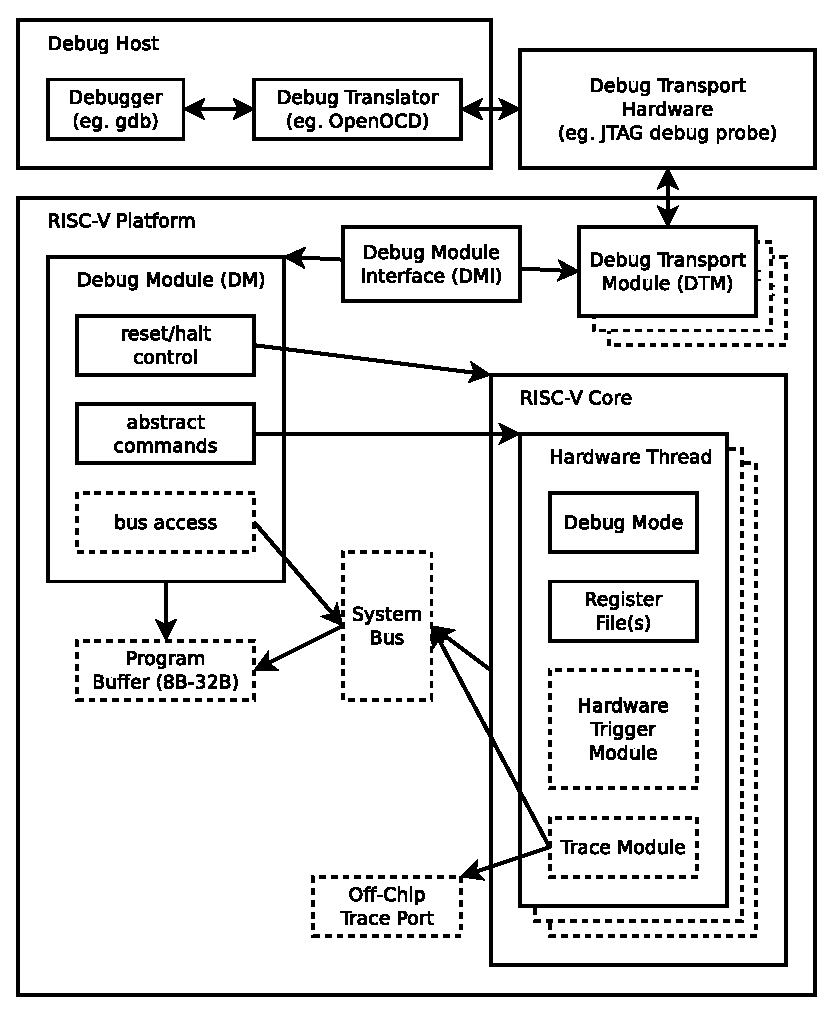
\includegraphics[width=\textwidth]{fig/overview.eps}
   \caption{RISC-V Debug System Overview}
   \label{fig:overview}
\end{figure}

The user interacts with the Debug Host (eg. laptop), which is running a
debugger (eg. gdb).  The debugger communicates with a Debug Translator (eg.
OpenOCD, which may include a hardware driver) to communicate with Debug
Transport Hardware (eg.  Olimex USB-JTAG adapter).
The Debug Transport Hardware connects the Debug Host to the Platform's Debug
Transport Module (DTM).  The DTM provides access to the DM using the Debug
Module Interface (DMI).

The DM allows the debugger to halt any hart in the platform. Abstract commands
provide access to GPRs and possibly other registers. More complex harts will
require the Program Buffer be implemented, which the debugger uses to have the
hart execute arbitrary instructions while halted.

Each RISC-V core may implement a Trigger Module for each hart.  These can
implement breakpoints, which cause a hart to halt spontaneously.  When that
happens the hart signals the DM that it is halted.
